\chapter{The Run-3 Operations of the CMS detector}
\label{chap:Ops}

The \ac{CMS} detector resumed data-taking in July 2022, following the start of the Run-3 of the \ac{LHC}. When compared to the Run-2, the center of mass energy of the proton beams increase from 13 TeV to 13.6 TeV in Run 3. At the same time, the peak instantaneous luminosity is kept at the same or higher level as the 2018 data-taking year ($2\times10^{34}~\textsf{cm}^{-2}\textsf{s}^{-1}$), as illustrated in Figure~\ref{fig:peak}.

\begin{figure}[tbh!]
 \begin{center}
 \begin{tabular}{c}
 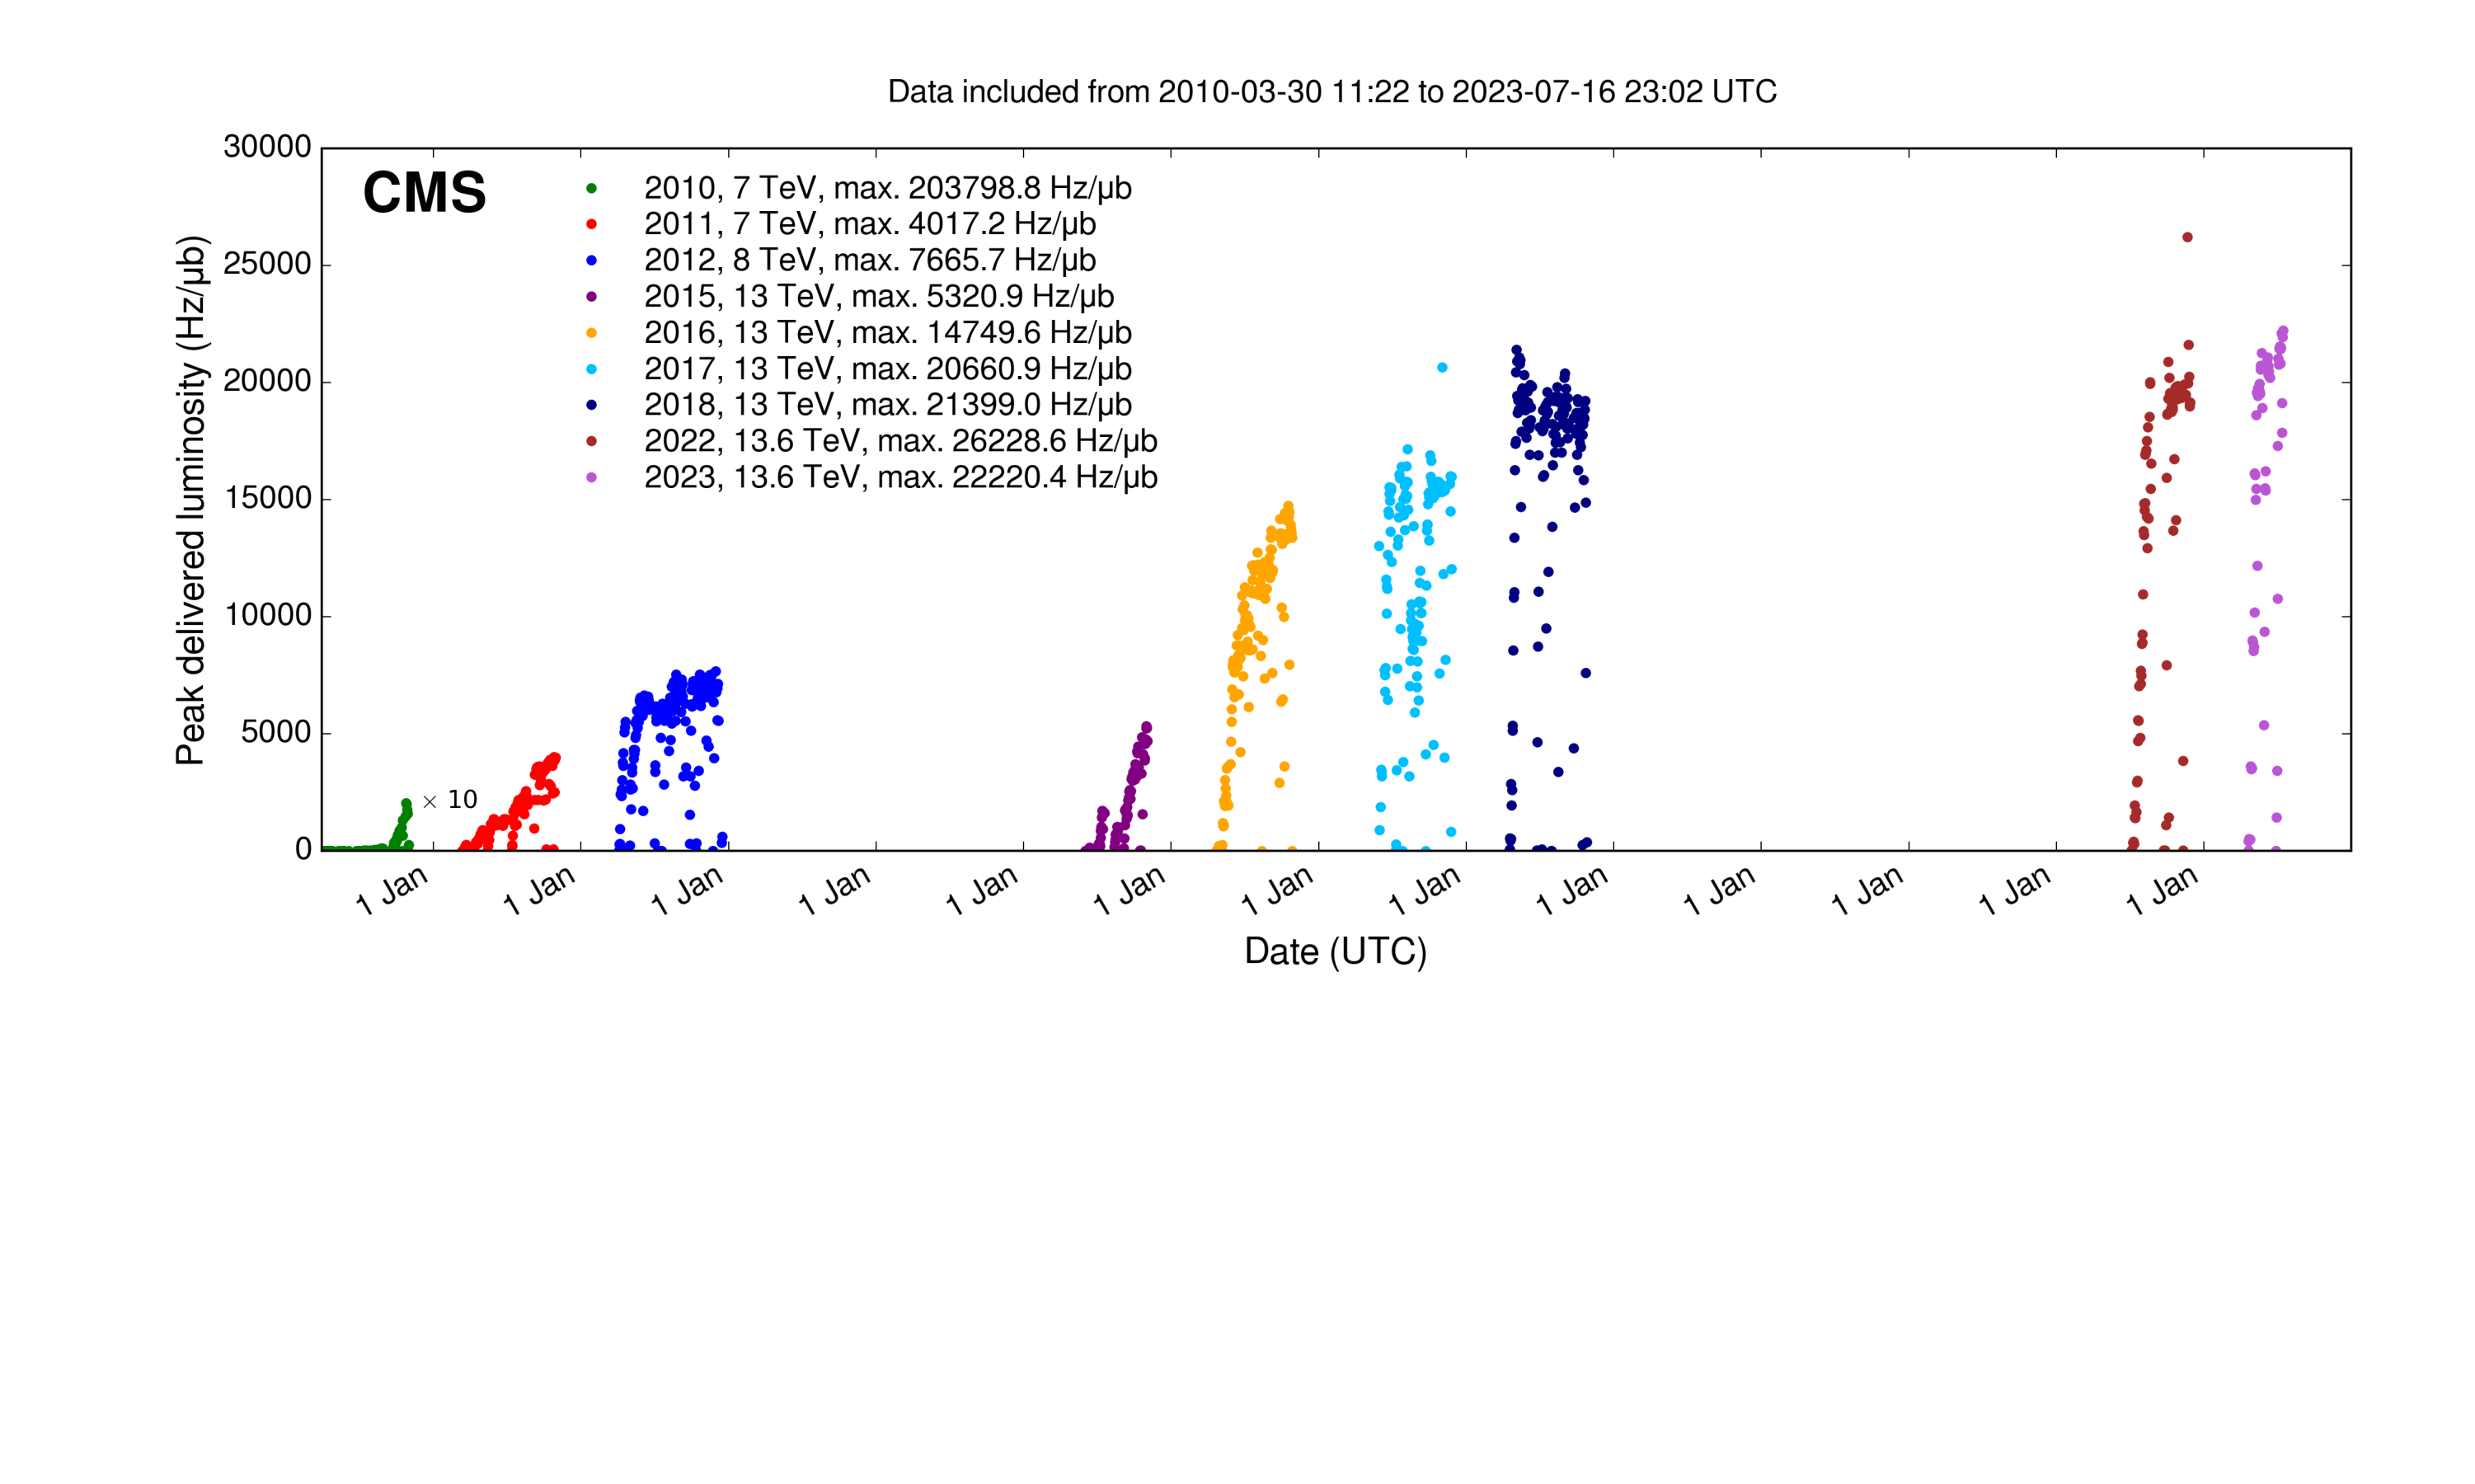
\includegraphics[width=\textwidth]{figures/Part2/Operation/peak_lumi_pp}
 \end{tabular}
 \caption{Peak luminosity versus day delivered to \ac{CMS} during stable beams and for proton-proton collisions, adapted from~\cite{twiki:lumi}.}
 \label{fig:peak}
 \end{center}
\end{figure}

Operations of the \ac{CMS} detector is coordinated by the \ac{CMS} Run Coordination, which is introduced in \autoref{sec:RC}. The \ac{CMS} control room is the commanding center of the \ac{CMS} operations, which is staffed 24$\times$7 during active data-taking period. Personnel who monitor and operate the \ac{CMS} detector from the control room are referred to as the ``central shift crew``, which is discussed further in \autoref{sec:ControlRoom}. In the In the context of detector operations, the principle contacts of the subsystems of the \ac{CMS} detector are known as the \ac{DOC} experts, or simply the \acp{DOC}. Core duties of one of the \acp{DOC}, the tracker \ac{DOC}, are described in \autoref{sec:DOC}.

\section{The CMS Run Coordination}
\label{sec:RC}

The \ac{CMS} detector is considered to be ``running'' when it is switched on and taking data. During this period, operations of various subsystems of the \ac{CMS} detector are controlled by the central shift crew. 

The Run Coordinators are responsible for the full scope of operations needed for the successful running of CMS. Strong cooperation with the Technical, Offline and Computing and Trigger Coordinators is required. Common areas of work occur in calibration and alignment, online database and trigger performance. Run Coordination is also responsible for monitoring aspects of data analysis coordination and the interaction with commissioning efforts in the Tracking, ECAL, HCAL, BRIL and Muon Detector Systems.

The Run Coordinators are responsible for the full scope of operations needed for the successful running of CMS. Strong cooperation with the Technical, Offline and Computing and Trigger Coordinators is required. Common areas of work occur in calibration and alignment, online database and trigger performance. Run Coordination is also responsible for monitoring aspects of data analysis coordination and the interaction with commissioning efforts in the Tracking, ECAL, HCAL, BRIL and Muon Detector Systems.

\section{Central Shift Crew}
\label{sec:ControlRoom}

The Run Coordinators are responsible for the full scope of operations needed for the successful running of CMS. Strong cooperation with the Technical, Offline and Computing and Trigger Coordinators is required. Common areas of work occur in calibration and alignment, online database and trigger performance. Run Coordination is also responsible for monitoring aspects of data analysis coordination and the interaction with commissioning efforts in the Tracking, ECAL, HCAL, BRIL and Muon Detector Systems.

The Run Coordinators are responsible for the full scope of operations needed for the successful running of CMS. Strong cooperation with the Technical, Offline and Computing and Trigger Coordinators is required. Common areas of work occur in calibration and alignment, online database and trigger performance. Run Coordination is also responsible for monitoring aspects of data analysis coordination and the interaction with commissioning efforts in the Tracking, ECAL, HCAL, BRIL and Muon Detector Systems.

\begin{figure}[tbh!]
 \begin{center}
 \begin{tabular}{c}
 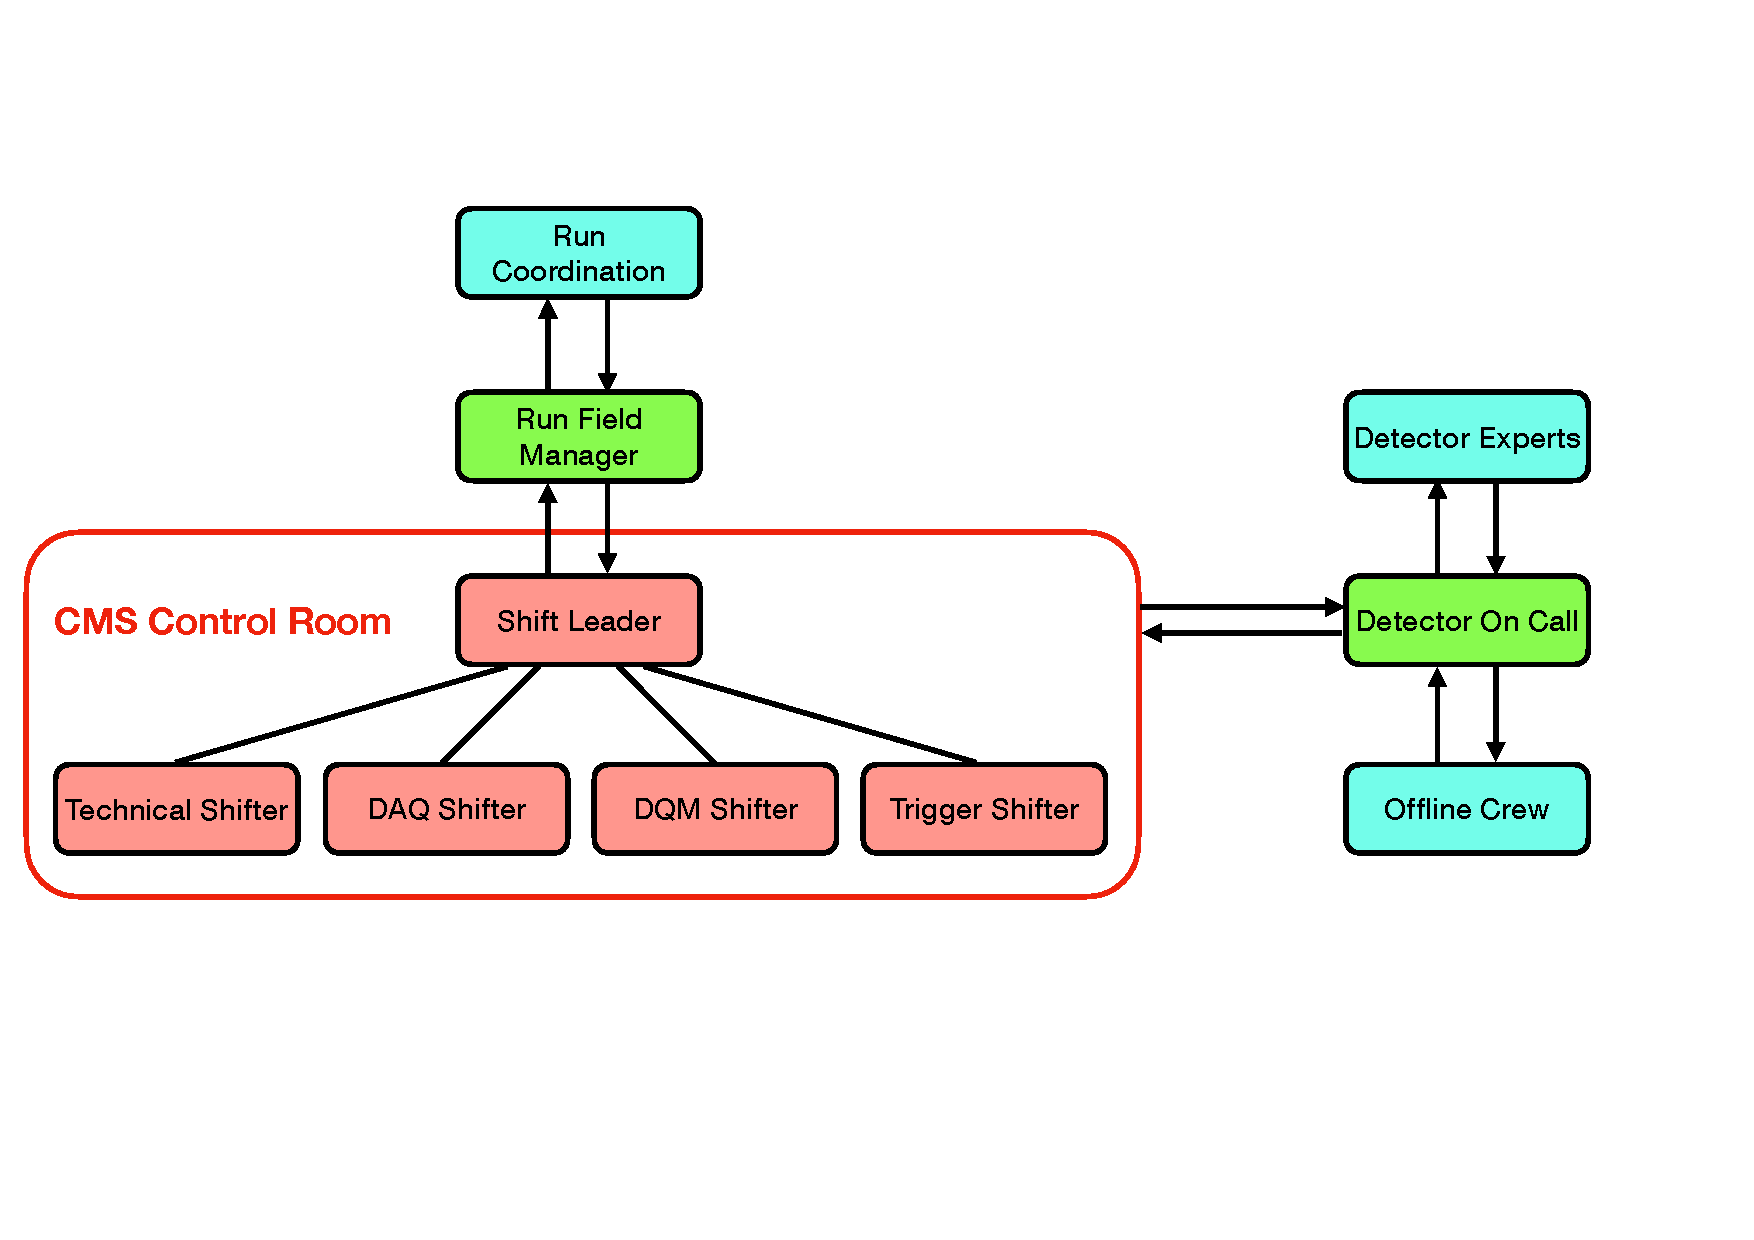
\includegraphics[width=0.9\textwidth]{figures/Part2/Operation/RC}
 \end{tabular}
 \caption{Main communication paths between various  the \ac{CMS} Run organization. The shift leader, technical, \ac{DAQ}, \ac{DQM}, and the trigger shifters are required to be present at the \ac{CMS} control room 24$\times$7. The \acp{RFM} and the \acp{DOC} are nominally present at the control room during the working hours. The Run Coordinators, subsystem expects, and offline shifters are not required to be at the control room although they often do.}
 \label{fig:RC}
 \end{center}
\end{figure}

The Run Coordinators are responsible for the full scope of operations needed for the successful running of CMS. Strong cooperation with the Technical, Offline and Computing and Trigger Coordinators is required. Common areas of work occur in calibration and alignment, online database and trigger performance. Run Coordination is also responsible for monitoring aspects of data analysis coordination and the interaction with commissioning efforts in the Tracking, ECAL, HCAL, BRIL and Muon Detector Systems.

\ac{DCS} \ac{DSS}

\section{Tracker Detector On-call Expert}
\label{sec:DOC}

One of the key goals of the \ac{CMS} tracker group is to ensure a stable and safe operation of the detector. This requires both well-trained operators as well as a modern \ac{DCS}. Built on top of the industrial product “WinCC”, the \ac{CMS} \ac{TCS}~\cite{Shah:2009zz,Karimeh:2020tzx} is designed to monitor the environmental conditions and safely operate the detector.

As part of the \ac{TCS} software, a \ac{FSM} toolkit is introduced. It is a powerful tool that assists operators in their daily job. It groups the power, cooling, dry gas and monitoring systems defined in the four \ac{TCS} projects in one hierarchical tree. The global state of the detector is continuously evaluated and made visible from the root Tracker FSM node giving critical information to the detector operator, as illustrated in Figure~\ref{fig:DCS}.

\begin{figure}[tbh!]
 \begin{center}
 \begin{tabular}{c}
 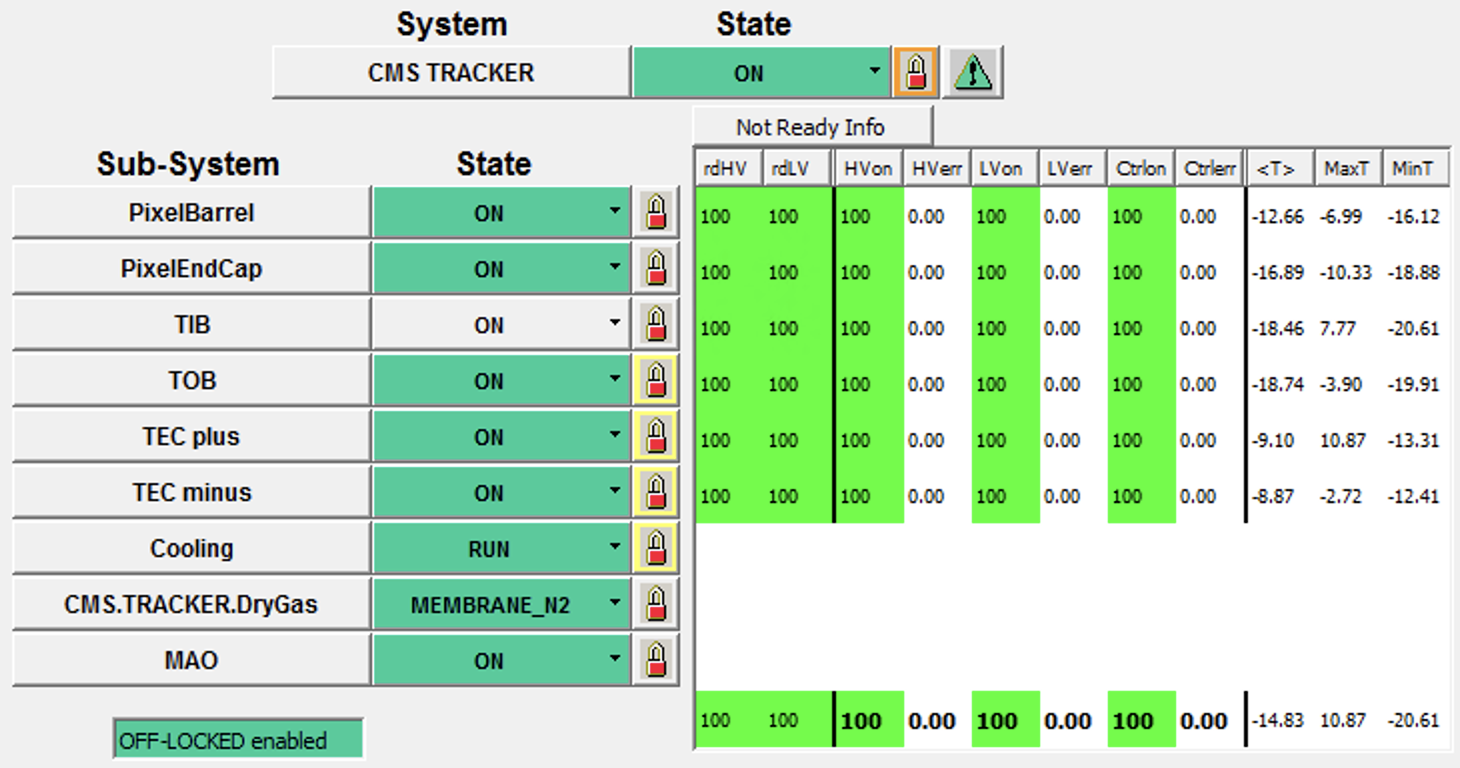
\includegraphics[width=0.8\textwidth]{figures/Part2/Operation/TrackerDCS}
 \end{tabular}
 \caption{Main panel of the tracker \ac{FSM}.}
 \label{fig:DCS}
 \end{center}
\end{figure}